\section{The model}
\label{sec:dsmc_model}
DSMC is a model that makes full use of statistical mechanics and the kinetic theory of gases. The physical system consists of $N$ atoms of the same type in a box with volume $V = L_xL_yL_z$ ($L_i$ being the length of the box in the $i'$th dimension) and porosity $\phi$ (the porosity was the fraction of the total volume available for fluids). The atoms all have mass $m$ and an effective diameter $d$. Instead of tracking the trajectory every single atom, we simulate $M$ particles, each representing $N_\text{eff}$ real atoms. We can interpret this approximation as that all atoms in a small region of space around the coordinates of a simulated particle move with approximately the same velocity. The system is periodic in all directions which means that $(L_x, L_y, L_z) = (0,0,0)$, the corners of the cube are the same point. If a particle passes through a boundary surface (one of the sides of the box), it will just enter at the opposite side, see figure \ref{fig:dsmc_periodic_boundary_conditions}.
\begin{figure}[ht]
\begin{center}
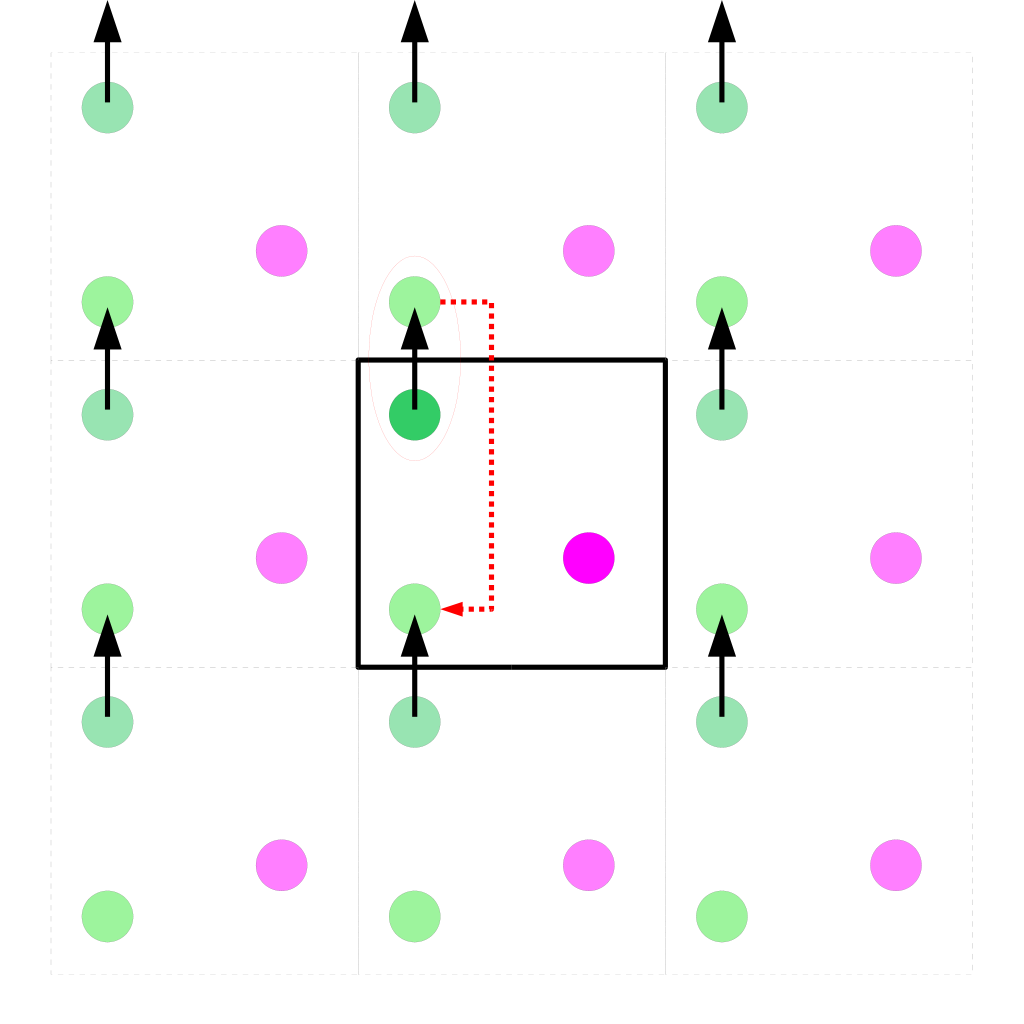
\includegraphics[width=0.7\textwidth, trim=0cm 0cm 0cm 0cm]{DSMC/figures/periodic_boundary_conditions.png}
\end{center}
\caption{Periodic boundary conditions allows particles to fly out of a system by re-entering it in the opposite side. This reduces the amount of finite size system effects. Image from \url{http://en.wikipedia.org/wiki/File:Limiteperiodicite.svg}, accessed 16 March, 2014.}
\label{fig:dsmc_periodic_boundary_conditions}
\end{figure}
The state of a DSMC simulation is fully described by the $6M$ phase variables, three velocities and three positions per simulated particle.

Since we don't have detailed information about the positions of all the real atoms, we cannot calculate the forces between the particles. Instead, we assume that the gas particles only undergo binary collisions (we neglect collisions between three or more particles), just like we did while deriving the Boltzmann equation in section \ref{sec:boltzmann_equation}. Particles are sorted into collision cells before the collisions are performed in a stochastic manner, where the rate of collisions and post-collision velocities are determined from kinetic theory. We can think that the collision step in the model is an operator, a stochastic function $\mathcal{C}(\vec r, \vec v, \mathcal{G})$, where $\vec r$ and $\vec v$ form the phase space point and $\mathcal G$ contains all information about the system geometry. Do not worry, this will be clear in a minute.\\
The equations of motion are integrated by applying the standard Euler method on the positions so that $\vec r_i(t+\Delta t) = \vec r_i(t) + \vec v_i(t)\Delta t$ for particle $i$. The timestep is chosen small enough so that we can split it into two parts; moving and colliding. This is a reasonable assumption as long as the timestep $\Delta t$ is smaller than the mean collision time $\tau_\text{coll}$ (equation \eqref{eq:kinetic_theory_mean_collision_time})
\begin{align}
	\Delta t \leq \tau_\text{coll} = \frac{1}{\sqrt 2 \pi d^2 \rho_n \langle v \rangle},
\end{align}
since the velocity then does not change during the timestep. If a particle interacts with a boundary during the timestep, some sort of surface interaction rule is applied before the timestep is continued (we allow a particle to collide with the surface several times during a single timestep).

The moving step can also be seen as a stochastic operator, $\mathcal{M}(\vec r, \vec v, \mathcal{G})$ since the surface interaction often is a stochastic process. Different surface interaction models are discussed in section \ref{sec:surface_interactions} with a detailed description of the implementation in section \ref{sec:dsmc_complex_geometries}. Statistical properties are sampled at the end of each timestep where the physical quantities are sampled as time averages. A flow chart illustrating the steps of a typical DSMC algorithm is presented in figure \ref{fig:dsmc_flowchart}.
\begin{figure}[ht]
\begin{center}
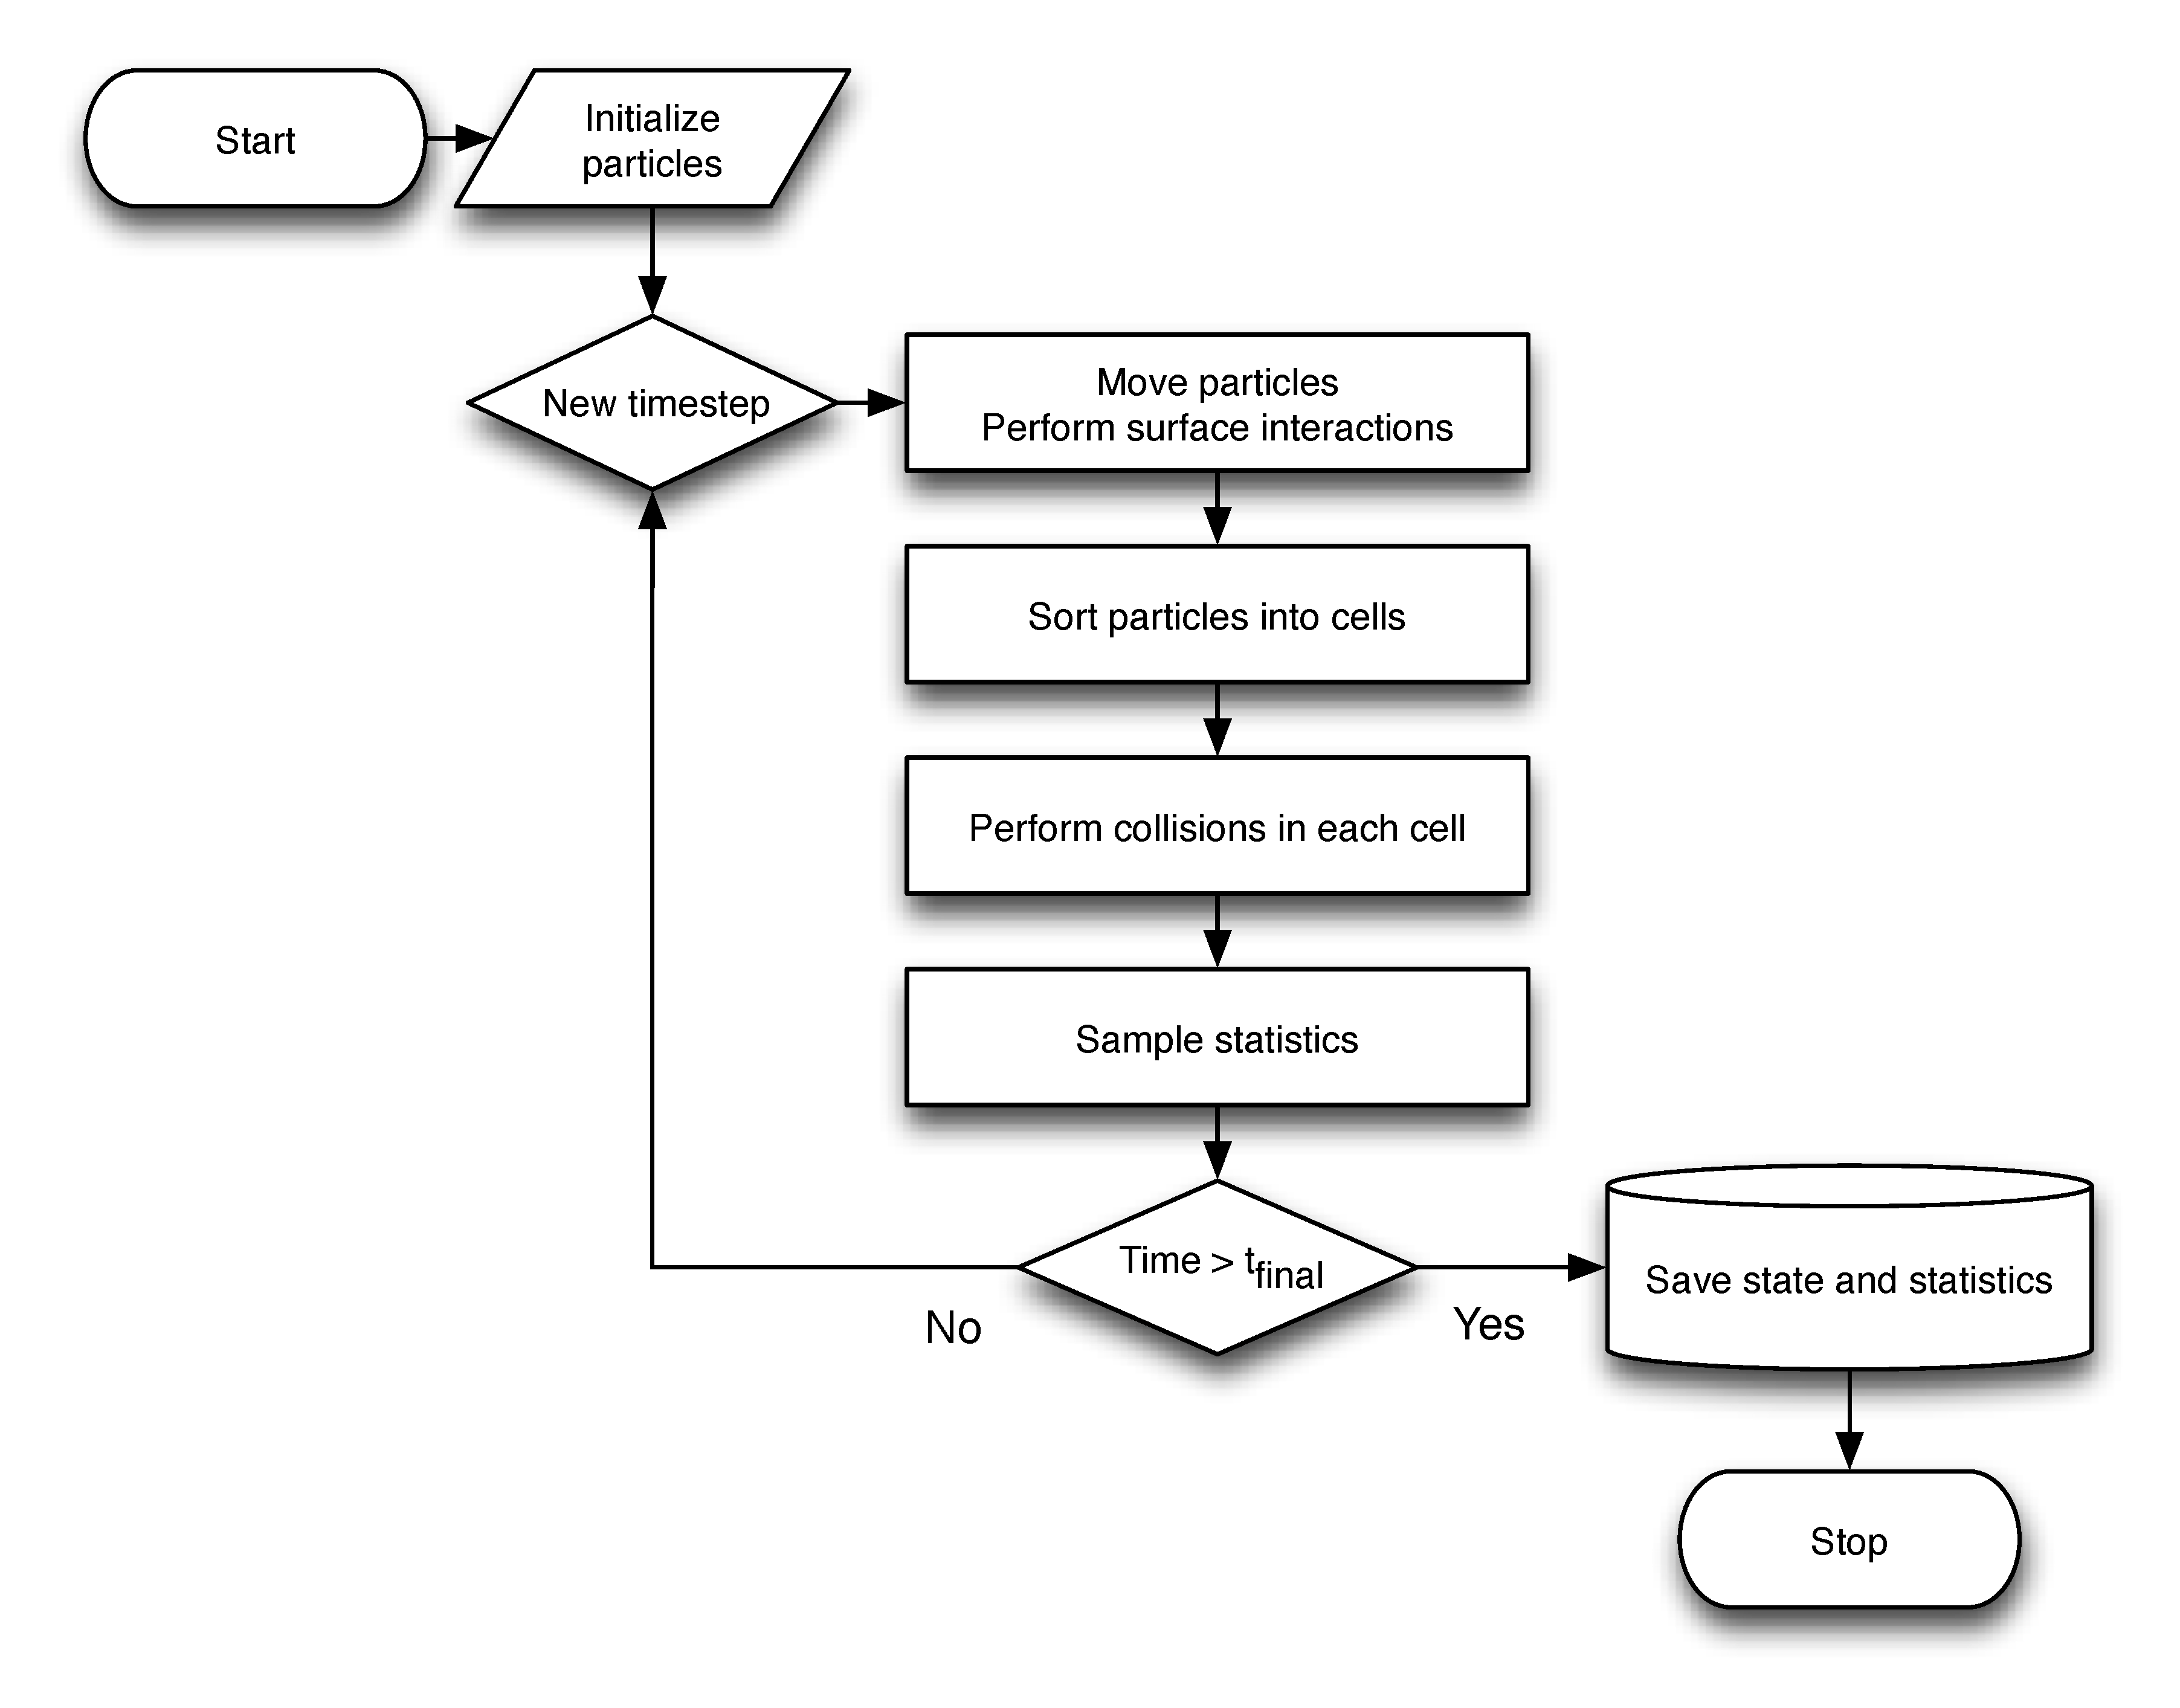
\includegraphics[width=\textwidth, trim=0cm 0cm 0cm 0cm, clip]{DSMC/figures/dsmc_flowchart.eps}
\end{center}
\caption{Typical steps for a DSMC algorithm.}
\label{fig:dsmc_flowchart}
\end{figure}


